\input setup_ueb
\begin{document}
\section*{Übungsaufgaben 1 \\
(Zahlen, Strings, Bedingungen, while-Schleifen)}

Hausaufgabe: Lösen Sie mindestens 6 der folgenden Aufgaben. Sie dürfen die
Aufgaben in Gruppen bearbeiten. Aufgaben mit Stern * zählen doppelt.

Abgabe im ISIS-Kurs, spätestes Abgabedatum wird dort angegeben, Gruppenpartner bitte bei der Abgabe vermerken.

Für einige Aufgaben benötigen Sie Zufallszahlen. Für Fließkomma-Zufallszahlen
zwischen 0 und 1 können Sie die Funktion \texttt{random} des Moduls \texttt{random} benutzen oder die Funktion \texttt{rand} des Moduls \texttt{numpy.random}.
Für ganze Zufallszahlen gibt es in den beiden Modulen eine Funktion \texttt{randint} (mit kleinen Unterschieden, sehen Sie sich help(...) an!).


\subsection*{Aufgaben aus dem Labor}

Diese Aufgaben kennt ihr vielleicht schon aus dem Mathesis-Kurs ... 

\begin{enumerate}[1.]

%\item \textbf{Mittlere Lebensdauer eines Bakteriums}

%Bestimmen Sie durch Simulation einen Näherungswert der Lebensdauer von
%Bakterien, die nach einem Zeitschritt mit Wahrscheinlichkeit $p$ sterben.

\item \textbf{Abstand von Fliegen auf einem Papier}

Zwei Fliegen landen zufällig (gleichverteilt) auf einem Quadrat der 
Seitenlänge  eins. Mit welcher Wahrscheinlichkeit ist der (euklidische) Abstand
der Fliegen größer als 1?
Ermitteln Sie einen Näherungswert durch eine Simulation
über eine Million Landungen. 

Gelingt es Ihnen, den Wert theoretisch zu bestimmen (technisch nicht so leicht)?


\item \textbf{Irrfahrt (2d)}

Simulieren mit Hilfe der Turtlegraphik ein Wesen, 
dass im Ursprung startet und in jedem Zeitschritt mit Wahrscheinlichkeit 1/4 
nach N/W/S/O läuft (eine gewisse Strecke s). 
Beende die Simulation, wenn das Wesen wieder im Ursprung ist.


Haben Sie Vermutungen darüber, mit welcher Wahrscheinlichkeit das Wesen überhaupt
zurückkehrt oder über die mittlere Dauer der Irrfahrt?   Wie könnten Sie solche
Hypothesen mit einer Simulation auf Plausibilität überprüfen? (Beweisen könnten
Sie sie allerdings nur mit Hilfe von Mathematik.)

%\item \textbf{Irrfahrt (2d), noch mal}

%Schreiben Sie diesmal ein Programm dass 2d-Irrfahrten nur berechnet und
%nicht zeichnet.  Simulieren Sie 1000 mal eine im Ursprung beginnende
%Irrfahrt von 10000 Schritten. Bestimmen Sie den mittleren Abstand
%vom Ursprung nach 10000 Schritten. (Sie müssen über den Mittelwert
%der 1000 Simulationen bilden.)

\item \textbf{Genomanalyse$^*$}
Lesen Sie mit dem folgenden Stück Code die ganze Datei \verb|protein_ecoli.txt| in einen
String. Es handelt sich um den Teil der DNA von E. Coli, der  das erste Protein (bezüglich
einer in den großen Gendatenbanken festgelegten Reihenfolge) codiert.
\begin{lstlisting}[language=Python]
f = open("protein_ecoli.txt", "r")
seq = ""

for line in f:
	seq = seq + line.rstrip()

f.close()
\end{lstlisting}
Schreiben Sie ein kleines Programm, das das längste Code-Stück sucht,
das (überschneidungsfrei) doppelt in dieser Sequenz vorkommt (oder alle längsten Stücke).


\item \textbf{Schere-Stein-Papier}

Schreiben Sie ein Programm, das gegen einen menschlichen Spieler  Schere-Stein-Papier
spielt.  Was würden Sie intuitiv für ein besonders gutes Programm gegen
einen Spieler halten, über den nichts bekannt ist, außer, dass er mit gewisser (unbekannter) Wahrscheinlichkeit eines
der drei Symbole zeigt, wenn das Ziel ist, möglichst oft zu gewinnen, egal was der
menschliche Spieler tut ? Können Sie beweisen, dass Sie die optimale Strategie gefunden haben ?

{\footnotesize
Diese einfache Aufgabe lässt sich als Ausgangspunkt für die Spieltheorie 
verwenden, indem man sie etwas weiter treibt.
Was ist  die optimale Strategie, wenn Siege nicht gleichviel zählen, sondern
eine Aus- oder Einzahlung stattfindet gemäß der folgenden Matrix ?

\begin{tabular}{ll| l l}
A & B & Ausz. an A & Ausz. an B\\ \hline
Schere & Papier & 2 & -2 \\
Papier & Stein  & 3 & -3 \\
Stein  & Schere & 1 & -1 \\
Papier & Schere & -2 & 2 \\
Stein & Papier & -3 & 3 \\
Schere & Stein & -1 & 1 \\
\end{tabular}

Zeigen beide das gleiche Symbol, erfolgt keine Auszahlung. Ein hierfür relevantes Stichwort aus der Spieltheorie 
lautet {\em beste gemischte Strategie} oder auch {\em Gleichgewicht gemischter Strategien}.

Frage zum Grübeln: Lässt sich die Strategie gegen einen {\em menschlichen} Spieler, der keine
Hilfsmittel benutzt,  verbessern  ?}


\item \textbf{Häufigkeit der Vokale}

Schreiben Sie ein Programm, das für einen String (also Text)
die Anzahl der 'e','a','i','o' und 'u' ermittelt. 
Sie können statt eines eingegebenen Strings auch einen 
ganzen Text verwenden.  Dazu kopieren Sie den Text
als Datei (auf ISIS stehen als Beispiele \texttt{das\_urteil.txt}
und \texttt{dickens\_martinchuzzlewit.txt} .)
in das Verzeichnis, wo sich ihr Programm befindet. Mit
\begin{lstlisting}[language=Python]
with open("das_urteil.txt","r") as f:
    text=f.read()
\end{lstlisting}
wird der ganze Text in dem String 'text' gespeichert.
Sie können daran etwa die Sprache erkennen, probieren Sie's aus.


\item \textbf{Ein Spiralornament}

Zeichnen Sie mit der Turtle ein spiralartiges Ornament
mit vierzig \glqq Umrundungen\grqq{}.
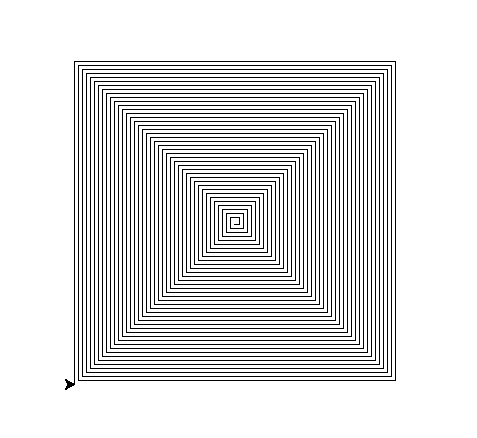
\includegraphics[width=0.5\textwidth]{spirale.png}



\item \textbf{Diskretes Räuber-Beute-Modell}

Dieses in der mathematischen Biologie betrachtete Modell beschreibt
die Entwicklung der Populationsdichte $x$ einer Beutespezies ('Kaninchen') und
der Populationsdichte $y$ einer Räuberspezies ('Füchse'). Die Populationen
werden nur in gewissen Zeitabständen ermittelt, und das Modell macht auch nur für diese Zeiten Voraussagen. Man sagt, das Modell sei {\em diskret in der Zeit}.

\[ x_{n+1} =  ax_n(1-x_n) - bx_ny_n \qquad y_{n+1} = cx_ny_n \;. \]

Schreiben Sie ein Programm, dass die Populationen mit den Parametern $a=3.5$, $b=2$, $c=4.05$ und den Anfangswerten
$x_0=0.5$ und $y_0=0.4$  hundert Schritte  lang berechnet und dabei $(x,y)$ mit turtle-Graphik visualisiert.

Sehen Sie sich die Bilder auch für andere Werte der Parameter an.


\end{enumerate}

%\item \textbf{Random-Walk}

%\end{enumerate}

\subsection*{Andere Aufgaben}

Einige Aufgaben sind einfach, einige schwieriger. Um was zu lernen solltet
ihr euch nicht nur solche Aufgaben suchen, die euch sehr einfach vorkommen.


\begin{enumerate}[1.]

\setcounter{enumi}{7}


\item \textbf{Buchstaben zu Bild}\\
Schreiben Sie ein Programm, das um die Eingabe einer Zeichenkette
aus den Buchstaben 'L','R' und 'G' bittet. Anschließend zeichnet
die Turtle-Graphik die Kurve, die durch die Anweisungen 'L' (nach links
drehen), 'R' (nach rechts drehen) und 'G' (50 Schritte geradeaus gehen)
gegeben ist, also liefert beispielsweise GLGLGLG ein Quadrat.

%\setcounter{enumi}{4}
%\item \textbf{Ein Kegel}\\ Schreiben Sie ein Programm, das als Eingabe den Radius $r$  und die
%Höhe $h$ eines Kegels einliest und das Volumen und die Oberfläche dieses
%Körpers ausgibt. (Sie können dazu die Konstante $\pi$ aus dem Modul \texttt{numpy}
%oder \texttt{math} importieren.)
\item \textbf{Eine quadratische Gleichung}\\ Schreiben Sie ein Programm, das die Koeffizienten $a$,$b$,$c$ einer
quadratischen Gleichung $ax^2+bx+c=0$ einliest und die reelle(n) Lösung(en) ausgibt,
bzw. gegebenenfalls eine Meldung, dass es keine reelle Lösung gibt.  
-- Schreiben Sie eine Variante, die die komplexen Lösungen ausgibt. In beiden
Fällen brauchen Sie die Wurzelfunktion \texttt{sqrt(x)}, die Sie wieder aus
\texttt{numpy} oder \texttt{math} importieren können. 
\item \textbf{Fakultät berechnen}\\ Schreiben Sie ein Programm, das eine natürliche Zahl einliest und
deren Fakultät ausgibt.
\item \textbf{Quersumme}\\
Schreiben Sie ein Programm, das als Eingabe eine Dezimalzahl erwartet
und die Quersumme ausgibt.
\item \textbf{Collatz-Folge}\\ Die Collatz-Folge $(a_n)_{n\in\N}$ zum Anfangswert $a_0\in \N$ ist wie folgt rekursiv definiert: Ist $a_n$ gerade, so ist $a_{n+1}=\frac{a_n}{2}$, andernfalls $a_{n+1}=3*a_n+1$.  Es ist nicht bekannt, ob diese Folge für alle Anfangswerte irgendwann bei $1$ ankommt (und anschließend periodische weitergeht $1\rightarrow 4 \rightarrow 2 \rightarrow 1 \rightarrow \cdots$.)
Schreiben Sie ein Programm, dass für einen eingebenen Anfangswerd die ersten 100
Folgenglieder ausgibt. Schreiben Sie anschließend eine Variante, die alle Glieder bis zur ersten $1$ und den Index dieser ersten $1$ ausgibt.  Schreiben Sie 
anschließend ein Programm, dass im Zahlenbereich bis zu 1 Million (oder gerne auch größer) den Anfangswert mit dem längsten Anfangsstück bis zur ersten $1$ ausgibt. 


\item \textbf{Verschl"usselung mit Caesarchiffre}

Bei der Caesarchiffre, einem einfachen Verfahren zur Verschl"usselung von
Nachrichten, ersetzt man die Buchstaben mit dem $n$. Nachfolger
im Alphabet (zyklisch), also z.B. f"ur $n = 3$ wird a zu d, b zu e, c zu f,
..., w zu z, x zu a, y zu b und z zu c. Aus \emph{eswarschondunkel}
wird dann \emph{hvzduvfkrqgxqnho}. 
(Traditionell verwendet man bei den einfachen Verschl"usselungen keine
Gro"s-/Kleinschreibung, Interpunktion und Leerzeichen -- das 
\glqq Knacken\grqq{} des Codes w"are sonst zu einfach. Ebenso k"onnen 
hier Umlaute und "s besser als ae, oe, ue und ss dargestellt werden.) 

Schreiben Sie ein Programm, das ein $n$ und den zu verschl"usselnden
Klartext einliest und daf"ur die verschl"usselte Zeichenkette ausgibt.


\item \textbf{Pseudozufallszahlen}\\
Wenn man in Programmen Zufallszahlen ben"otigt, so werden meist Folgen
von Pseudozufallszahlen verwendet, d.h. eine Folge von Zahlen 
$a_1, a_2, a_3, \ldots$, die f"ur statistische Analysen wie das Ergebnis 
eines Zufallsprozesses aussehen.
Ein ein\-fa\-ches Beispiel solcher Pseudozufallfolgen mit Folgegliedern 
aus dem Bereich von 0 bis 65535 erh"alt man durch
$a_{i+1} = (25173 a_i + 13849) \% 65536$.
(Dies ist eine "ubliche Weise f"ur die Definition von Zahlenfolgen: 
Die Gleichung gibt an, wie man aus einem Folgeglied $a_i$ das n"achste 
Folgeglied $a_{i+1}$ errechnet.) 
Schreiben Sie ein Programm, das das erste Folgeglied (den \emph{seed})
vom Nutzer einliest und die n"achsten 20 Folgeglieder
ausgibt.   \\
Zusatz: Veranschaulichen sie die Zufallszahlen, indem Sie durch diese
Zahlen die Bewegung einer \texttt{turtle} steuern. Dafür gibt
es verschiedene Möglichkeiten, lassen Sie sich was einfallen.
Wenn das Ergebnis schön wirr aussieht, scheint der Zufall zufällig genug
zu sein.

\item \textbf{Primzahltest}\\Schreiben Sie ein Programm, das eine natürliche Zahl einliest und 
prüft, ob es sich um eine Primzahl handelt.

% \item \textbf{Simulation eines Zerfallsprozesses}\\
% Schreiben Sie ein Programm, das die mittlere Lebensdauer 
% von Lebwesen, die in einem Zeitschritt mit Wahrscheinlichkeit 
% $p=1/6$ sterben, simuliert.\\
% Hinweis:  Für die Simulation des Zufalls können
% Sie eine Funktion des Pakets \texttt{random} verwenden.  Importieren
% Sie am Anfang Ihres Programms das Paket wie folgt
% \begin{verbatim}
% import random
% \end{verbatim}
% Wenn Sie nun \texttt{a$=$random.random()} setzen, so bekommt
% die Variable $a$ einen zufällig zwischen $0$ und $1$ gewählten 
% Wert. (Die Werte sind nicht wirklich zufällig, sondern wie oben durch
% einen 'Pseudozufallszahlengenerator' erzeugt; für die meisten 
% Zwecke, auch komplexe physikalische Simulationen, ist das
%  aber zufällig genug.)
%\item \textbf{Pseudozufallszahlen}\\
%Wenn man in Programmen Zufallszahlen ben"otigt, so werden meist Folgen
%von Pseudozufallszahlen verwendet, d.h. eine Folge von Zahlen 
%$a_1, a_2, a_3, \ldots$, die f"ur statistische Analysen wie das Ergebnis 
%eines Zufallsprozesses aussehen.
%Ein ein\-fa\-ches Beispiel solcher Pseudozufallfolgen mit Folgegliedern 
%aus dem Bereich von 0 bis 65535 erh"alt man durch
%$a_{i+1} = (25173 a_i + 13849) \% 65536$.
%(Dies ist eine "ubliche Weise f"ur die Definition von Zahlenfolgen: 
%Die Gleichung gibt an, wie man aus einem Folgeglied $a_i$ das n"achste 
%Folgeglied $a_{i+1}$ errechnet.) 
%Schreiben Sie ein Programm, das das erste Folgeglied (den \emph{seed})
%vom Nutzer einliest und die n"achsten 20 Folgeglieder
%ausgibt.
\item \textbf{Klammerung pr"ufen}\\
Schreiben Sie ein Programm, das f"ur eine Zeichenkette "uberpr"uft, ob
die enthaltenen (runden) Klammern den Regeln einer korrekten
Klammerung folgen. Dazu muss f"ur jede "offnende Klammer
\glqq\texttt{(}\grqq{} eine nachfolgende schlie"sende Klammer
\glqq\texttt{)}\grqq{} existieren und es darf keine schlie"sende
Klammer ohne vorhergehende "offnende Klammer dazu vorkommen. Andere
Zeichen als die runden Klammern sollen einfach ignoriert werden.

Beispielsweise korrekt geklammert sind \p{'()'},\p{''}, \p{'(()(a)(
  ()((b))))'}, nicht korrekt \p{'(()'} und \p{'a (()()) b)'}.

\item \textbf{Harshad-Zahlen}\\
Eine nat"urliche Zahl hei"st Harshad-Zahl, wenn sie durch ihre Quersumme (bezüglich der Dezimalschreibweise) teilbar ist. Beispielsweise ist f"ur $777$ die Quersumme $7+7+7=21$ und teilt $777$.
Schreiben Sie ein Programm, dass die Harshard-Zahlen von 1 bis 100 berechnet.
\item \textbf{Palindrom} 
Schreiben Sie zwei Programme, die einen String einlesen und prüfen,
ob es sich um ein Palindrom handelt: 1. ein einzeiliges Programm, das ohne
Schleifen auskommt und die besonderen String-Operationen verwendet. 2. ein Programm,
das mit Schleifen arbeitet.
\end{enumerate}

\subsection*{Mehr Turtle}

Hier noch einige Aufgaben, die Turtlegraphik verwenden.


\begin{enumerate}
\setcounter{enumi}{18}
\item \textbf{regelmäßiges Polygon}\\
Schreiben Sie ein Programm, das um Eingabe einer (natürlichen) Zahl n 
bittet und anschließend  mit der Turtle-Graphik ein n-Eck zeichnet.
\item \textbf{Stern}\\
Schreiben Sie ein Programm, das um Eingabe einer Zahl n 
bittet und anschließend einen n-zackigen Stern zeichnet.
\item \textbf{Mäander}\\
Schreiben Sie ein Programm, das nach Eingabe einer Zahl n 
ein n-fach wiederholtes Mäander-Ornament zeichnet (s.  (s. \texttt{https://de.wikipedia.org/wiki/Mäander\_(Ornamentik)}).
\end{enumerate}


\end{document}
